\chapter{Generaci�n de reportes}
\section{ReporTool}
La segunda parte del trabajo consisti� en la realizaci�n de reportes sobre el tr�fico capturado por el sniffer.
Nosotros construimos una herramienta que denominamos reporTool. La misma permite realizar los distintos analisis de trafico (reportes) generando una salida en formato pdf o en formato html mediante una interfaz grafica.

\begin{figure}[H]
\centering
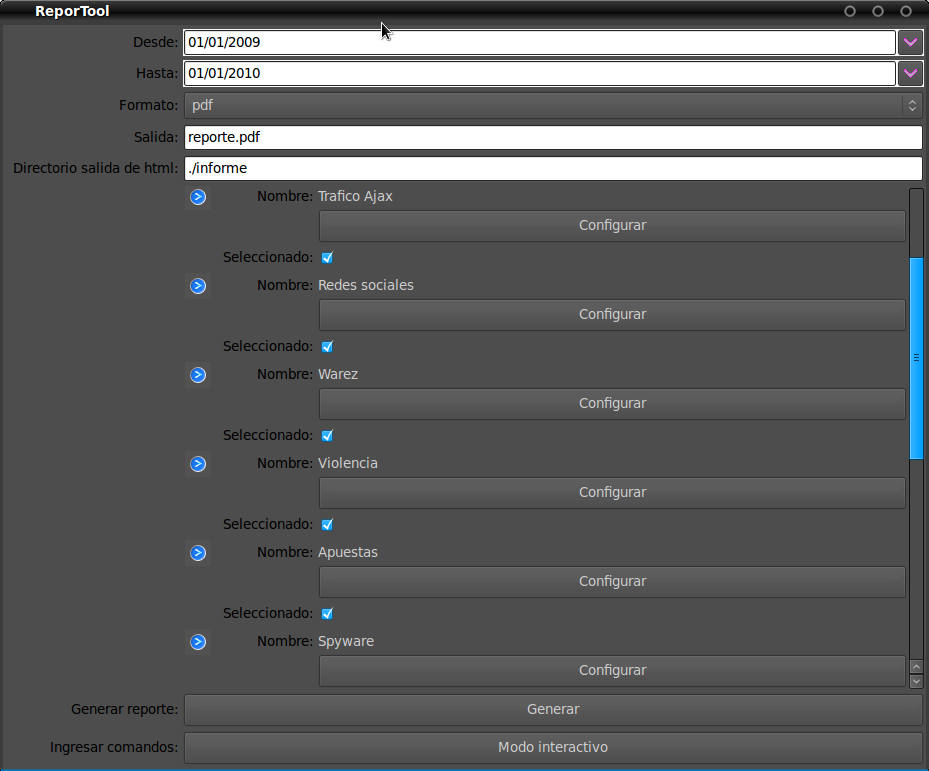
\includegraphics[scale=0.4]{./figuras/Pantallazo.png}
\caption{Captura de pantalla de reporTool}
\end{figure}

En las siguientes secciones daremos una breve descripci�n de los reportes por nosotros realizados. Posteriormente explicaremos el modo interactivo que presenta la herramienta y finalmente mostraremos como es posible agregar reportes propios para ser corridos con reporTool.

\section{Reportes}
Los siguientes son los reportes incluidos con reporTool

\subsection{Reporte de horario laboral}
Este reporte permite analizar el tr�fico discriminandolo seg�n un periodo laboral (d�as de la semana, y rango horario). De esta manera el reporte puede mostrar que usuarios usaron internet fuera de dichos horarios y que porcentaje de su actividad estuvo en infracci�n. El reporte puede mostrar todos los pedidos que se realizaron fuera de hora o solo mostrar el porcentaje en infracci�n.

Ademas puede mostrar la distribuci�n del uso de internet a lo largo de las distintas horas del d�a.

\subsection{Reporte por blacklists}
Este reporte permite especificar en un archivo una lista negra con dominios. El reporte analiza el tr�fico buscando visitas a alguno de esos dominios. Es en verdad una familia de reportes, ya que es posible utilizar varias instancias del mismo utilizando distintas blacklists, con distintos tipos de dominios, por ejemplo sitios de apuestas, de warez, etc. 

Si bien reporTool trae unos archivos de blacklists para ciertas categorias, es f�cil modificar esas blacklist, o reemplazarlas por otras, crear un reporte nuevo que trabaje con blacklists de otras categorias.

Estas son las blacklists inclu�das con reporTool:
%TODO: listar las blackslists que se incluyen en la entrega

Los siguientes son sitios donde es posible descargar blacklists de distintas categorias:
\begin{itemize}
\item \verb_http://squidguard.mesd.k12.or.us/_
\item \verb_http://www.shallalist.de/_
\item \verb<http://cri.univ-tlse1.fr/documentations/cache/squidguard_en.html#contrib<
\item \verb_http://urlblacklist.com/?sec=download_
\end{itemize}

Este reporte puede generar graficos de cantidad de infracciones por usuarios, que porcenteja del tr�fico por usuario y total esta en infracci�n, cuales son los sitios de la blacklist mas visitados, entre otras cosas.

\subsection{Reporte de tr�fico AJAX}
%TODO: sergio completa esto

\subsection{Reporte por content type}
En este reporte podemos ver el tipo de contenido del tr�fico, basicamente hicimos seis separaciones distintas (audio, video, aplicaci�n, multipart, imagen y texto). En el reporte podemos ver, por ejemplo, la cantidad de tr�fico de tipo imagen y la cantidad de tr�fico que no es imagen. Tambi�n tenemos la cantidad de tr�fico de imagen separada por usuario para poder ver mas en detalle que hace cada usuario.

\begin{figure}[H]
\centering

\includegraphics[scale=0.4]{./figuras/multimedia.png}
\caption{Captura de pantalla de reporTool}
\end{figure}


Si bien se podr�an hacer varias separaciones mas (como por ejemplo discriminar por tr�fico de tipo jpeg o pdf) estas separaciones generales nos parecieron las mas interesantes para mostrar en el reporte.
Igualmente el sniffer no escapa a la posibilidad de querer hacer algunas de estas consultas y lo podemos hacer en el modo interactivo (o extendiendo el reporte).

\subsection{Reporte por tr�fico de nivel de aplicaci�n}
%TODO: victoria complete esto por favor :D

\subsection{Reporte de tr�fico global}
%TODO: sergio completa esto, o si queres lo hago yo, pero comete un paty

\subsection{Reporte de seguimiento}
Este reporte permite elegir hasta 5 sitios y analizar la evoluci�n de la cantidad de visitas y de tr�fico mes a mes para estos sitios, a lo largo de un periodo de tiempo determinado.

\subsection{Reporte por heuristica}
Este reporte puede pensarse de alguna forma como un complemento para el reporte por blacklists. El mismo utiliza un archivo donde se definen ciertas keywords (por ejemplo, keywords sobre apuestas: poker, black jack, casino, etc) que son buscadas en las requests y en los responses. El reporte muestra luego para que usuarios se encontraron matches, asi como cuales fueron los principales matches.

Las blacklists solo encuentran requests a los dominios en ellos definidos, entonces es factible que un usuario pueda visitar alguna p�gina que no esta en la blacklist pero que deber�a estarlo, o que incluso saltee el chequeo de las blacklists (por ejemplo navegando con la cache de google). La busqueda heuristica permite detectar estas cosas, al costo de posiblemente dar falsos positivos sobre el contenido de las visitas. Sin embargo puede ser una herramienta util para detectar usos indebidos.

\section{Modo interactivo}
Ademas de la posibilidad de realizar reportes, reporTool provee un mecanismo interactivo para realizar consultas a la base de datos. En vez de brindar una interfaz para simplemente ejecutar SQL en la base de datos, lo cual es posible con cualquier cliente de bases de datos; brindamos una consola python con ciertos elementos de alto nivel, brindados por el ORM que permiten interactuar con la base de datos.

Para obtener una sesion, se debe utilizar el comando get\_session. Una vez que tenemos una sesion, podemos realizar queries sobre las clases que mapean a la base de datos (presentadas anteriormente) mediante la interfaz que provee sqlalchemy. 

Para mas informacion se puede consultar:

\begin{itemize}
\item \verb<http://www.sqlalchemy.org/docs/05/session.html#querying<
\item \verb<http://www.sqlalchemy.org/docs/05/reference/orm/query.htmlz<
\end{itemize}

A continuaci�n presentamos un ejemplo de como obtener las requests originadas en la IP 10.0.2.17:

\framebox{\begin{minipage}[t][1\totalheight]{1\columnwidth}%
\noindent
\ttfamily
\shorthandoff{"}\\
\hlstd{Python\ }\hlnum{2.6.2\ }\hlstd{}\hlsym{(}\hlstd{release26}\hlsym{{-}}\hlstd{maint}\hlsym{,\ }\hlstd{Apr\ }\hlnum{19\ 2009}\hlstd{}\hlsym{,\ }\hlstd{}\hlnum{01}\hlstd{}\hlsym{:}\hlstd{}\hlnum{56}\hlstd{}\hlsym{:}\hlstd{}\hlnum{41}\hlstd{}\hlsym{)}\hspace*{\fill}\\
\hlstd{}\hlsym{{[}}\hlstd{GCC\ }\hlnum{4.3.3}\hlstd{}\hlsym{{]}\ }\hlstd{on\ linux2\hspace*{\fill}\\
Type\ }\hlstr{``help''}\hlstd{}\hlsym{,\ }\hlstd{}\hlstr{``copyright''}\hlstd{}\hlsym{,\ }\hlstd{}\hlstr{``credits''}\hlstd{\ }\hlkwa{or\ }\hlstd{}\hlstr{``license''}\hlstd{\ }\hlkwa{for\ }\hlstd{more\ information}\hlsym{.}\hspace*{\fill}\\
\hlstd{}\hlsym{$>$$>$$>$\ }\hlstd{s\ }\hlsym{=\ }\hlstd{}\hlkwd{get\textunderscore session}\hlstd{}\hlsym{()}\hspace*{\fill}\\
\hlstd{}\hlsym{$>$$>$$>$\ }\hlstd{q\ }\hlsym{=\ }\hlstd{s}\hlsym{.}\hlstd{}\hlkwd{query}\hlstd{}\hlsym{(}\hlstd{RequestHTTP}\hlsym{)}\hspace*{\fill}\\
\hlstd{}\hlsym{$>$$>$$>$\ }\hlstd{reqs\ }\hlsym{=\ }\hlstd{q}\hlsym{.}\hlstd{}\hlkwb{filter}\hlstd{}\hlsym{(}\hlstd{RequestHTTP}\hlsym{.}\hlstd{ipOrigen\ }\hlsym{==\ }\hlstd{}\hlstr{``10.0.2.17''}\hlstd{}\hlsym{).}\hlstd{}\hlkwd{all}\hlstd{}\hlsym{()}\hlstd{}\hspace*{\fill}\\
\mbox{}
\normalfont
\shorthandon{"}

\end{minipage}}

Tambi�n es posible ejecutar queries sobre la base con sintaxis sql, mediante la utilizaci�n del engine, sin embargo para utilizar SQL es conveniente usar el cliente propio del motor de la base de datos. El siguiente ejemplo permite obtener todas las requests (el resultado es un ResultProxy):

\framebox{\begin{minipage}[t][1\totalheight]{1\columnwidth}%

\noindent
\ttfamily
\shorthandoff{"}\\
\hlstd{Python\ }\hlnum{2.6.2\ }\hlstd{}\hlsym{(}\hlstd{release26}\hlsym{{-}}\hlstd{maint}\hlsym{,\ }\hlstd{Apr\ }\hlnum{19\ 2009}\hlstd{}\hlsym{,\ }\hlstd{}\hlnum{01}\hlstd{}\hlsym{:}\hlstd{}\hlnum{56}\hlstd{}\hlsym{:}\hlstd{}\hlnum{41}\hlstd{}\hlsym{)}\hspace*{\fill}\\
\hlstd{}\hlsym{{[}}\hlstd{GCC\ }\hlnum{4.3.3}\hlstd{}\hlsym{{]}\ }\hlstd{on\ linux2\hspace*{\fill}\\
Type\ }\hlstr{``help''}\hlstd{}\hlsym{,\ }\hlstd{}\hlstr{``copyright''}\hlstd{}\hlsym{,\ }\hlstd{}\hlstr{``credits''}\hlstd{\ }\hlkwa{or\ }\hlstd{}\hlstr{``license''}\hlstd{\ }\hlkwa{for\ }\hlstd{more\ information}\hlsym{.}\hspace*{\fill}\\
\hlstd{}\hlsym{$>$$>$$>$\ }\hlstd{con\ }\hlsym{=\ }\hlstd{engine}\hlsym{.}\hlstd{}\hlkwd{connect}\hlstd{}\hlsym{()}\hspace*{\fill}\\
\hlstd{}\hlsym{$>$$>$$>$\ }\hlstd{con}\hlsym{.}\hlstd{}\hlkwd{execute}\hlstd{}\hlsym{(}\hlstd{}\hlstr{``select\ {*}\ from\ requests''}\hlstd{}\hlsym{)}\hlstd{}\hspace*{\fill}\\
\mbox{}
\normalfont
\shorthandon{"}


\end{minipage}}

Para mas informaci�n puede consultarse:

\verb<http://www.sqlalchemy.org/docs/05/reference/sqlalchemy/connections.html<

\section{Agregado de nuevos reportes}
ReporTool fue pensado para ser facilmente extensible, es decir que sea facil poder agregar nuevos reportes definidos por el usuario.

Para poder definir un nuevo reporte, es necesario definir una clase que herede de Reporte. Esta misma debe implementar el metodo ejecutar que recibe un desde y un hasta, que son las fechas entre las cuales debe analizarse el tr�fico.

Dicho metodo debe devolver un string latex, que es el que se utilizar� para generar el pdf o el html correspondiente al reporte.

Una vez definida esta clase, debe importarse en reporTool, crear una instancia, envolverla con un Configurador y agregar al configurador a la lista de configuradores.
 
Para ilustrar un poco mejor esto, presentaremos un ejemplo muy sencillo de como se define y se agrega un nuevo reporte.

\subsection{Definici�n de la clase}
Creamos un nuevo archivo llamado reporteTrucho.py, en el ponemos:

\framebox{\begin{minipage}[t][1\totalheight]{1\columnwidth}%

\noindent
\ttfamily
\shorthandoff{"}\\
\hlstd{}\hlkwa{from\ }\hlstd{reporte\ }\hlkwa{import\ }\hlstd{Reporte}\hspace*{\fill}\\
\hlkwa{from\ }\hlstd{latex\ }\hlkwa{import\ }\hlstd{LatexFactory}\hspace*{\fill}\\
\hlkwa{from\ }\hlstd{enthought}\hlsym{.}\hlstd{traits}\hlsym{.}\hlstd{api\ }\hlkwa{import\ }\hlstd{}\hlsym{{*}}\hspace*{\fill}\\
\hlstd{}\hlkwa{from\ }\hlstd{enthought}\hlsym{.}\hlstd{traits}\hlsym{.}\hlstd{ui}\hlsym{.}\hlstd{api\ }\hlkwa{import\ }\hlstd{}\hlsym{{*}}\hspace*{\fill}\\
\hlstd{}\hspace*{\fill}\\
\hlkwa{class\ }\hlstd{}\hlkwd{ReporteTrucho}\hlstd{}\hlsym{(}\hlstd{Reporte}\hlsym{):}\hspace*{\fill}\\
\hlstd{\hspace*{\fill}\\
}\hlstd{\ \ \ \ }\hlstd{flagTrucho\ }\hlsym{=\ }\hlstd{}\hlkwd{Bool}\hlstd{}\hlsym{(}\hlstd{}\hlkwa{True}\hlstd{}\hlsym{)}\hspace*{\fill}\\
\hlstd{}\hlstd{\ \ \ \ }\hlstd{rangoTrucho\ }\hlsym{=\ }\hlstd{}\hlkwd{Range}\hlstd{}\hlsym{(}\hlstd{}\hlnum{1}\hlstd{}\hlsym{,}\hlstd{}\hlnum{10}\hlstd{}\hlsym{,}\hlstd{}\hlnum{5}\hlstd{}\hlsym{)}\hspace*{\fill}\\
\hlstd{\hspace*{\fill}\\
}\hlstd{\ \ \ \ }\hlstd{}\hlkwa{def\ }\hlstd{}\hlkwd{ejecutar}\hlstd{}\hlsym{(}\hlstd{self}\hlsym{,}\hlstd{desde}\hlsym{,}\hlstd{hasta}\hlsym{):}\hspace*{\fill}\\
\hlstd{}\hlstd{\ \ \ \ \ \ \ \ }\hlstd{l\ }\hlsym{=\ }\hlstd{}\hlkwd{LatexFactory}\hlstd{}\hlsym{()}\hspace*{\fill}\\
\hlstd{}\hlstd{\ \ \ \ \ \ \ \ }\hlstd{l}\hlsym{.}\hlstd{}\hlkwd{chapter}\hlstd{}\hlsym{(}\hlstd{}\hlstr{``Reporte\ Trucho''}\hlstd{}\hlsym{)}\hspace*{\fill}\\
\hlstd{}\hlstd{\ \ \ \ \ \ \ \ }\hlstd{l}\hlsym{.}\hlstd{}\hlkwd{texto}\hlstd{}\hlsym{(}\hlstd{}\hlstr{``\%s''}\hlstd{}\hlsym{\%}\hlstd{self}\hlsym{.}\hlstd{flagTrucho}\hlsym{)}\hspace*{\fill}\\
\hlstd{}\hlstd{\ \ \ \ \ \ \ \ }\hlstd{}\hlkwa{return\ }\hlstd{l}\hlsym{.}\hlstd{}\hlkwd{generarOutput}\hlstd{}\hlsym{()}\hlstd{}\hspace*{\fill}\\
\mbox{}
\normalfont
\shorthandon{"}
        
\end{minipage}}

Analicemos un poco el codigo:
La primera l�nea importa la clase Reporte, para que el reporte que queremos definir pueda heredar de dicha clase.

Luego se importa la clase LatexFactory que brinda algunas funciones para poder generar codigo latex mas facilmente.

Las l�nes 3 y 4 son necesarias para importar la libreria traits que permite generar luego de forma automatica la GUI para modificar el reporte.

Luego comienza la definici�n de la clase. Las dos primeras lineas de la definicion, establecen dos atributos que va a tener el reporte, un flag booleano que por default vale True y un rango que va del 1 al 10 y que por default comienza en 5. Estos atributos se podran luego modificar mediante la interfaz grafica.

Luego se define el metodo ejecutar como dijimos anteriormente. En este caso se devuelve un capitulo latex con el titulo \textit{Reporte trucho} y un texto que muestra el valor del flag.

Ya tenemos definida la clase del nuevo reporte, vamos a agregarlo. En rerpoTool.py agregamos las siguientes lineas:

\framebox{\begin{minipage}[t][1\totalheight]{1\columnwidth}%

\noindent
\ttfamily
\shorthandoff{"}\\
\hlstd{}\hlslc{\#\#\#\#\#\#\#\ Imports\ de\ los\ distintos\ reportes\ \#\#\#\#\#\#\#}\hspace*{\fill}\\
\hlstd{}\hlkwa{from\ }\hlstd{horarioLaboral\ }\hlkwa{import\ }\hlstd{FueraDeHorario}\hspace*{\fill}\\
\hlkwa{from\ }\hlstd{blackList\ }\hlkwa{import\ }\hlstd{ListaNegra}\hspace*{\fill}\\
\hlkwa{from\ }\hlstd{ajax\ }\hlkwa{import\ }\hlstd{Ajax}\hspace*{\fill}\\
\hlkwa{from\ }\hlstd{contentType\ }\hlkwa{import\ }\hlstd{ContentType}\hspace*{\fill}\\
\hlkwa{from\ }\hlstd{nonHTTP\ }\hlkwa{import\ }\hlstd{NonHTTP}\hspace*{\fill}\\
\hlkwa{from\ }\hlstd{evolucion\ }\hlkwa{import\ }\hlstd{EvolucionMensual}\hspace*{\fill}\\
\hlkwa{from\ }\hlstd{heuristica\ }\hlkwa{import\ }\hlstd{Heuristica}\hspace*{\fill}\\
\hlkwa{from\ }\hlstd{traficoEnGral\ }\hlkwa{import\ }\hlstd{TraficoEnGral}\hspace*{\fill}\\
\hspace*{\fill}\\
\hlkwa{from\ }\hlstd{reporteTrucho\ }\hlkwa{import\ }\hlstd{ReporteTrucho\ }\hlslc{\#Agregamos\ esta\ linea}\hlstd{}\hspace*{\fill}\\
\mbox{}
\normalfont
\shorthandon{"}

\end{minipage}}

De esta manera, importamos nuestro reporte, para que este disponible.

\framebox{\begin{minipage}[t][1\totalheight]{1\columnwidth}%

\noindent
\ttfamily
\shorthandoff{"}\\
\hlstd{}\hlslc{\#\#\#\#\#\#\#\#\#\#\#\#\#\#\#\#\#\#\#\#\#\#\#\#\#\#\#\#\#\#\#\#\#\#\#\#\#\#\#\#\#\#\#\#\#\#\#\#\#\#\#\#\#\#\#}\hspace*{\fill}\\
\hlstd{}\hlslc{\#\#}\hlstd{\ \ \ \ \ \ }\hlslc{Otros\ reportes\ definidos\ por\ el\ usuario}\hlstd{\ \ \ \ \ \ \ }\hlslc{\#}\hspace*{\fill}\\
\hlstd{}\hlslc{\#\#\#\#\#\#\#\#\#\#\#\#\#\#\#\#\#\#\#\#\#\#\#\#\#\#\#\#\#\#\#\#\#\#\#\#\#\#\#\#\#\#\#\#\#\#\#\#\#\#\#\#\#\#\#}\hspace*{\fill}\\
\hlstd{rt\ }\hlsym{=\ }\hlstd{}\hlkwd{ReporteTrucho}\hlstd{}\hlsym{()}\hspace*{\fill}\\
\hlstd{configDePrueba\ }\hlsym{=\ }\hlstd{}\hlkwd{Configurador}\hlstd{}\hlsym{(}\hlstd{script\ }\hlsym{=\ }\hlstd{rt}\hlsym{,\ }\hlstd{nombre}\hlsym{=}\hlstd{}\hlstr{``Reporte\ Trucho''}\hlstd{}\hlsym{,}\hlstd{descripcion\ }\hlsym{=\ }\hlstd{}\hlstr{``Soy\ un\ reporte\ muy\ trucho''}\hlstd{}\hlsym{)}\hlstd{}\hspace*{\fill}\\
\mbox{}
\normalfont
\shorthandon{"}

\end{minipage}}

En este codigo, creamos la instancia de reporte, y lo wrappeamos en un configurador. Un configurador es lo que permite mostrar el nombre del reporte y los botones para seleccionar al reporte y para configurarlo.

\framebox{\begin{minipage}[t][1\totalheight]{1\columnwidth}%

\noindent
\ttfamily
\shorthandoff{"}\\
\hlstd{}\hlslc{\#\#\#\#\#\#\#\#\#\#\#\#\#\#\#\#\#\#\#\#\#\#\#\#\#\#\#\#\#\#\#\#\#\#\#\#\#\#\#\#\#\#\#\#\#\#\#\#\#\#\#\#\#\#}\hspace*{\fill}\\
\hlstd{configuradores}\hlsym{={[}}\hlstd{c}\hlsym{,}\hlstd{c1}\hlsym{,}\hlstd{c2}\hlsym{,}\hlstd{c3}\hlsym{,}\hlstd{c4}\hlsym{,}\hlstd{c5}\hlsym{,}\hlstd{c6}\hlsym{,}\hlstd{c7}\hlsym{,}\hlstd{c8}\hlsym{,}\hlstd{c9}\hlsym{,}\hlstd{c10}\hlsym{,}\hlstd{c11}\hlsym{,}\hlstd{c12}\hlsym{{]}}\hspace*{\fill}\\
\hlstd{}\hspace*{\fill}\\
\hspace*{\fill}\\
\hlslc{\#\#\ Registrar\ en\ esta\ lista\ los\ configuradores\ definidos\ por\ el\ usuario}\hspace*{\fill}\\
\hlstd{configuradores}\hlsym{.}\hlstd{}\hlkwd{append}\hlstd{}\hlsym{(}\hlstd{configDePrueba}\hlsym{)}\hlstd{}\hspace*{\fill}\\
\mbox{}
\normalfont
\shorthandon{"}

\end{minipage}}

Aqu� agregamos el configurador a la lista de configuradores de reporTool.

Finalmente si ejecutamos reporTool, vemos que el reporte ya esta listo para ejecutarse:

\begin{figure}[H]
\centering
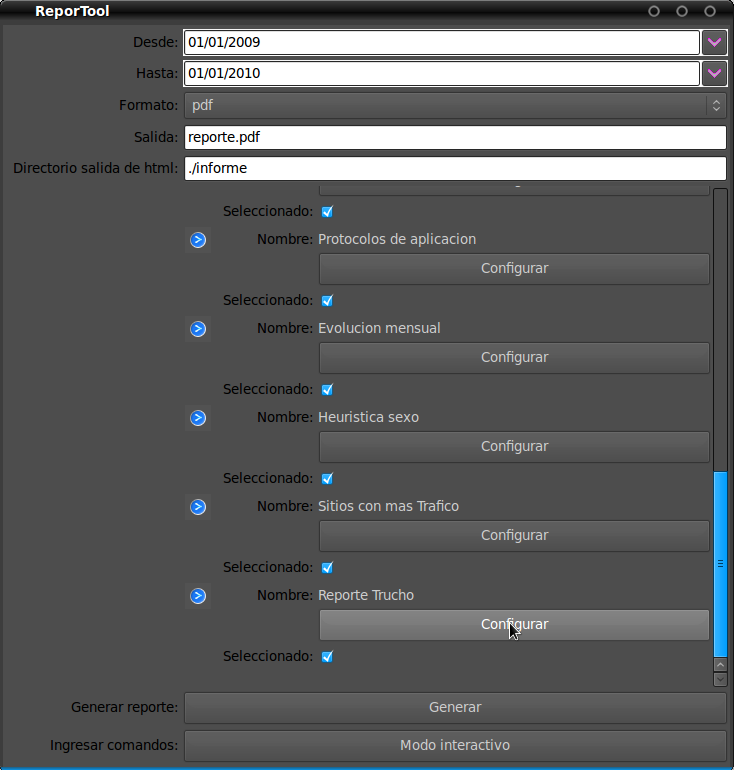
\includegraphics[scale=0.5]{./figuras/reporteAgregado.png}
\end{figure}
